%% Template for a preprint Letter or Article for submission
%% to the journal Nature.
%% Written by Peter Czoschke, 26 February 2004
%%


\documentclass{nature}
\usepackage{amsmath,amssymb}
\usepackage{hyperref}
\usepackage{cite}
\usepackage{graphicx}
\usepackage{algorithm, algpseudocode}
\usepackage{xr}
\externaldocument{nature-methods}
%\graphicspath{ {figures/} }
\newcommand*{\bigcdot}{\raisebox{-0.25ex}{\scalebox{1.2}{$\cdot$}}}

%% make sure you have the nature.cls and naturemag.bst files where
%% LaTeX can find them

\bibliographystyle{naturemag}

\title{Neuron's Eye View: Inferring Features of Complex Stimuli from Neural Responses \\ Supplementary Information}

%% Notice placement of commas and superscripts and use of &
%% in the author list

\author{Xin (Cindy) Chen$^{1,3}$, Jeffrey M. Beck$^{2, 3}$ \& John M. Pearson$^{1, 3}$}


\begin{document}

\maketitle

\begin{affiliations}
 \item Duke Institute for Brain Sciences, Duke University, Durham, North Carolina, USA
 \item Department of Neurobiology, Duke University Medical Center, Durham, North Carolina, USA
 \item Center for Cognitive Neuroscience, Duke University, Durham, North Carolina, USA
\end{affiliations}


\section*{Derivation of Evidence Lower Bound (ELBO)}
Here we derive the evidence lower bound (ELBO) used as a variational objective by our inference algorithm. That is, we want to calculate
\begin{equation}
    \mathcal{L} \equiv \mathbb{E}_q \left[\log \frac{p(\Theta|N)}{q(\Theta)} \right] = \mathbb{E}_q \left[\log p(\Theta|N) \right] + \mathcal{H}[q(\Theta)]
\end{equation}
From \cite{beal2003variational}, this can be written
\begin{multline}
    \mathcal{L} = \mathbb{E}_{q(\pi)} \left[\log \frac{p(\pi)}{q(\pi)} \right]
    + \mathbb{E}_{q(A)} \left[\log \frac{p(A)}{q(A)} \right]
    + \mathbb{E}_{q}\left[ \log \frac{p(N, z|\lambda, A, \pi)}{q(z)}\right] \\
    + \mathbb{E}_{q(\theta)} \left[\log \frac{p(\theta)}{q(\theta)} \right]
    + \mathbb{E}_{q(\lambda)} \left[\log \frac{p(\lambda)}{q(\lambda)} \right]
    + \mathbb{E}_{q(\gamma)} \left[\log \frac{p(\gamma)}{q(\gamma)} \right]
\end{multline}
For the first two terms, updates are standard and covered in \cite{beal2003variational}. The rest we do piece-by-piece below:

\subsection{Log evidence.}
\label{sec:log_evidence}
We would like to calculate $\mathbb{E}_{q}\left[ \log \frac{p(N, z|x, \Theta)}{q(z)}\right]$. To do this, we make use of expectations calculated via the posteriors returned from the forward-backward algorithm
\begin{align}
    \xi_{t} &\equiv p(z_{t}|N, \theta) &
    \Xi_{t, ij} &\equiv p(z_{t+1} = j, z_{t} = i|N, \theta) &
    \log Z_{t} &= \log p(N_{t+1}|N_{t}, \Theta)
\end{align}
Here, we have suppressed the latent feature index $k$ and abuse notation by writing the observation index as $t$, but in the case of multiple observations at a given time, we pool across units and presentations: $N_t \equiv \sum_{m; t(m) = t} N_m$. From this, we can write
\begin{multline}
    \label{eq:log_evidence}
     \mathbb{E}_{q}\left[ \log p(N, z|x, \Theta) \right] =
     \sum_{mkr} \left[N_m \left(
        \overline{\log \theta_m} + \overline{\log \lambda_{0u(m)}} +
        \xi_{t(m)k}\overline{\log \lambda_{zuk}} +
        x_{t(m)r} \overline{\log \lambda_{xu(m)r}}
     \right) \right] \\
     - \sum_m \overline{\theta_m} \mathbb{E}_q\left[\Lambda_{t(m)u(m)} \right]
      + \sum_{tk} \left[ \text{tr}\left(\Xi_{tk} \overline{\log A_k^T} \right)
     + \xi_{0k}^T \overline{\log \pi_k}
     \right]
    + \text{constant}
 \end{multline}
In what follows, we will drop the irrelevant constant. For $\overline{\log y}$, where $y \in \lbrace \theta, \lambda_0, \lambda_z, \lambda_x \rbrace$, the assumption $q(y) = \text{Ga}(\alpha, \beta)$ gives
\begin{equation}
    \overline{\log y} = \psi(\alpha) - \log \beta
\end{equation}
with $\psi(x)$ the digamma function. Likewise, the expectation $\overline{\theta}$ is straightforward. For the expectation of the rate, we have
\begin{equation}
    \label{eff_rate}
    \mathbb{E}_q\left[
        \lambda_{0u} \prod_k (\lambda_{zuk})^{z_{tk}} \prod_r (\lambda_{xur})^{x_{tr}}
    \right] = \frac{\alpha_{0u}}{\beta_{0u}}
    \prod_k \left(1 - \xi_{tk} + \xi_{tk} \frac{\alpha_{zuk}}{\beta_{zuk}} \right)
    \prod_r \frac{1}{\beta_{xur}^{x_{tr}}} \frac{\Gamma(\alpha_{xur} + x_{tr})}{\Gamma(\alpha_{xur})}
\end{equation}
However, for $\alpha \gg x$, we have $\Gamma(\alpha + x)/\Gamma(\alpha) \approx \alpha^x$, so that we can write
\begin{equation}
    \label{HFG}
    \mathbb{E}_q[\Lambda_{tu}] = H_{0u} F_{tu} G_{tu}
\end{equation}
with $G_{tu} \approx \prod_r (\alpha_{xur}/\beta_{xur})^{x_{tr}}$. In addition, it will later be useful to have the expectation over \emph{all except} a particular feature $k$ or $r$, for which we define
\begin{align}
    \label{F}
    F_{tuk} &\equiv \prod_{k'\neq k} \left(1 - \xi_{tk'} + \xi_{tk'} \frac{\alpha_{zuk'}}{\beta_{zuk'}} \right) \\
    \label{G}
    G_{tur} &\equiv \prod_{r' \neq r} \left(\frac{\alpha_{xur'}}{\beta_{xur'}} \right)^{x_{tr'}}
\end{align}
Finally, we want the entropy of the variational posterior over $z$, $\mathbb{E}_q[-\log q(z)]$. We can write this in the form
\begin{equation}
    -\sum_{tk} \left[
        \xi_{tk}^T\eta_{tk} + \text{tr}\left(\Xi_{tk} \tilde{A}_k^T \right)
        + \xi_{0k}^T\tilde{\pi}_k
        - \log Z_{tk}
    \right]
\end{equation}
with $(\eta, \tilde{A}, \tilde{\pi})$ the parameters of the variational posterior corresponding to the emission, transition, and initial state probabilities of the Markov chain (interpreted as matrices) and $Z$ the normalization constant. From \cite{beal2003variational}, we have that variational updates should give
\begin{align}
    \tilde{A}_k &\leftarrow \overline{\log A_k} &
    \tilde{\pi}_k &\leftarrow \overline{\log \pi_k}
\end{align}
while the effective emission probabilities in the ``on'' ($z = 1$) state of the HMM are
\begin{align}
    \eta_{tk} &\leftarrow \delta_{z_{tk}, 1} \sum_{m; t(m) = t} N_m \overline{\log \lambda_{zu(m)k}}
    - \sum_{m; t(m) = t} \overline{\theta_m} H_{0u(m)} F_{tku(m)} G_{tu(m)}
\end{align}
Given these update rules, we can then alternate between calculating $(\eta, \tilde{A}, \tilde{\pi})$, performing forward-backward to get $(\xi, \Xi, \log Z)$ and recalculating $(\eta, \tilde{A}, \tilde{\pi})$.

\subsection{Overdispersion, firing rate effects.}
Both the case of $p(\theta)$ and $p(\lambda)$ are straightforward. If we ignore subscripts and write $p(y) = \text{Ga}(a, b)$, $q(y) = \text{Ga}(\alpha, \beta)$, then
\begin{equation}
    \mathbb{E}_q \left[\log \frac{p(y)}{q(y)} \right] =
    (\overline{a} - 1) \overline{\log y} + \overline{b} \overline{y} + \mathcal{H}[q(y)]
\end{equation}
where again, $\overline{\log y}$, $\overline{y}$ and $\mathcal{H}[q(y)]$ are straightforward properties of the Gamma distribution. Expectations of the prior parameters are listed in Table \ref{expectation_table}. Note in the last line that there is no expectation, since we have not assumed a hierarchy over firing rate effects for the covariates, $x$.

\begin{table}[ht]
\caption{Expectations of prior parameters for overdispersion and firing rates}
\label{expectation_table}
\begin{center}
\begin{tabular}{lcc}
\multicolumn{1}{c}{\bf Variable}  &\multicolumn{1}{c}{\bf $\mathbb{E}_q[a]$} &\multicolumn{1}{c}{\bf $\mathbb{E}_q[b]$}
\\ \hline
$\theta$ &$\overline{s}$ &$\overline{s}$ \\
$\lambda_0$ &$\overline{c_0}$ &$\overline{c_0 d_0}$ \\
$\lambda_z$ &$\overline{c_z}$ &$\overline{c_z d_z}$ \\
$\lambda_x$ &$a_x$ &$b_x$ \\
\end{tabular}
\end{center}
\end{table}

\subsection{Hyperparameters.}
As shown in the main text, the hyperparameters $c$ and $d$, given gamma priors, have conjugate gamma posteriors, so that their contribution to the evidence lower bound, $\mathbb{E}_q \left[\log \frac{p(\gamma)}{q(\gamma)} \right]$ is a sum of terms of the form
\begin{align}
    (a_{c} - 1) \overline{\log c} + b_{c} \overline{c} + \mathcal{H}[q(c)] +
    (a_{d} - 1) \overline{\log d} + b_{d} \overline{d} + \mathcal{H}[q(d)]
\end{align}
In other words, these are straightforward gamma expectations, functions of the prior parameters $a$ and $b$ for each variable and the corresponding posterior parameters $\alpha$ and $\beta$. Similarly, the overdispersion terms are exactly the same with the substitutions $c \rightarrow s$, $d\rightarrow 1$.

As we will see below, the expectations under the variational posterior of $s$, $c$, and $d$ are themselves straightforward to calculate.

\subsection{Autocorrelated noise.}
In the main text, we assumed the $\theta_m$ to be uncorrelated. However, it is possible to model temporal autocorrelation among the $\theta_m$ when observations correspond to the same neuron at successive time points. More specifically, let us replace the observation index $m$ by $\tau$, the experimental clock time. We then write a particular observation as corresponding to a stimulus time $t(\tau)$ and a set of units $u(\tau)$, which, for simplicity, we will assume fixed and simply write as $u$.\footnote{The generalization to partially overlapping neurons and stimuli is straightforward but complex and notationally cumbersome.} To model the autocorrelation of noise across successive times, we then write
\begin{align}
    N_{m} &\sim \text{Pois}(\Lambda_{t(\tau), u} \theta_{\tau u}) &
    \text{Assuming } \theta_{\tau u} = \phi_{\tau u} \theta_{\tau - 1, u}
\end{align}

If $\phi_{0u} = \theta_{0u}$, we then have $\theta_{\tau u} = \prod_{\tau' \le \tau} \phi_{\tau' u}$. In essence, this is a log-autoregressive process in which the innovations are not necessarily normally distributed. In fact, if we further assume that $p(\phi_{\tau u}) = \mathrm{Ga}(s_u, r_u)$ and $q(\phi_{\tau u}) = \mathrm{Ga}(\omega_{\tau u}, \zeta_{\tau u})$, we can once again make use of conjugate updates.

Given these assumptions, we need to make the following modifications for the third and fifth terms in the evidence lower bound of Eq (\ref{eq:log_evidence}):
\begin{align}
    \sum_{mkr} N_m \xi_{t(m)k}\overline{\log \lambda_{zuk}} &\rightarrow
        \sum_{mkr} N_m \xi_{t(m)k}\overline{\log \lambda_{zuk}} +
        \sum_{\tau u} \overline{\log\phi_{\tau u}} \sum_{\tau' \ge \tau} N_{\tau' u} \\
    - \sum_m \overline{\theta_m} \mathbb{E}_q\left[\Lambda_{t(m)u(m)} \right] &\rightarrow
        - \sum_{\tau u} H_{0u} F_{\tau ku} G_{\tau u} \prod_{\tau' \le \tau} \frac{\omega_{\tau' u}}{\zeta_{\tau' u}}
\end{align}

Thus the effective emission probabilities in State 1 now become:
\begin{align}
    \eta_{tk} &\rightarrow \delta_{z_{tk}, 1} \sum_{m} N_m \overline{\log \lambda_{zuk}}
    - \sum_{u; t(\tau) = t} H_{0u} F_{\tau ku} G_{\tau u} \prod_{\tau' \le \tau} \frac{\omega_{\tau' u}}{\zeta_{\tau' u}}
\end{align}


\subsection{Latent states, semi-Markov dynamics.}

We model each of the latent states $z_{tk}$ as an independent Markov process for each feature $k$. That is, each $k$ indexes an independent Markov chain with initial state probability $\pi_k\sim \text{Dir}(\alpha_\pi)$ and transition matrix $A_k\sim \text{Dir}(\alpha_A)$. For the semi-Markov case, we assume that the dwell times in each state are distributed independently for each chain according to an integer-valued, truncated lognormal distribution with support on the integers $1\dots D$:
\begin{align}
    \label{semi-markov}
    p_k(d|z = j) &= \text{Log-Normal}(d|m_{jk}, s^2_{jk}) / W_{jk}  \\
    W_{jk} &= \sum_{d = 1}^D \text{Log-Normal}(d|m_{jk}, s^2_{jk})
\end{align}
Note that we have allowed the dwell time distribution to depend on both the feature $k$ and the state of the Markov chain $j$. In addition, we put independent Normal-Gamma priors on the mean $(m_{kj})$ and precision $(\tau_{kj} \equiv s_{kj}^{-2})$ parameters of the distribution: $(m, \tau) \sim \text{NG}(\mu, \lambda, \alpha, \beta)$.

In this case, we additionally need to perform inference on the parameters $(m, \tau)$ of the dwell time distributions for each state. In the case of continuous dwell times, our model in Equation \ref{semi-markov} would have $W = 1$ and be conjugate to the Normal-Gamma prior on $(m, \tau)$, but the restriction to discrete dwell times requires us to again lower bound the variational objective:
\begin{equation}
    \mathbb{E}_q\left[-\log W_{jk} \right] =
    \mathbb{E}_q\left[- \log \left( \sum_{d=1}^D p(d|j)\right) \right]
    \ge -\log \sum_{d = 1}^D \mathbb{E}_q\left[p(d|j)\right]
\end{equation}
This correction for truncation must then be added to $\mathbb{E}_q[p(z|\Theta)]$. For inference in the semi-Markov case, we use an extension of the forward-backward algorithm\cite{Yu2006-bb}, at the expense of computational complexity $\mathcal{O}(SDT)$ $(S = 2)$ per latent state, to calculate $q(z_k)$. For the $4SK$ hyperparameters of the Normal-Gamma distribution, we perform an explicit BFGS optimization on the $4S$ parameters of each chain on each iteration (detailed in Subsection \ref{semimarkovdd}).


\section*{Inference}
\subsection{hierarchical priors.}
As stated in the Methods section, for the latent states and baselines, we assume hierarchical priors. This allows us to model each neuron's firing rate response to a particular stimulus as being drawn from a population response to that same stimulus. We also assume that the moment-to-moment noise in firing rates, $\theta_m$, follows a neuron-specific distribution. As a result of the form of this hierarchy given in Eq (\ref{hierarchy}) of main article, the first piece in Eq (\ref{elbo}) of main article contains multiple terms of the form
\begin{equation}
    \mathbb{E}_q \left[\sum_u \log p(\lambda_u|c, d)\right] = \sum_u \mathbb{E}_q \left[
    (c - 1) \log \lambda_u - cd\lambda_u + c \log cd - \log \Gamma(c)
    \right]
\end{equation}
In order to calculate the expectation, we make use of the following inequality \cite{abramowitz1964handbook}
\begin{equation}
    \sqrt{2\pi} \le \frac{z!}{z^{z+\frac{1}{2}} e^{-z}} \le e
\end{equation}
to lower bound the negative gamma function and approximate the above as
\begin{equation}
    \log p(\lambda) \ge \sum_u \left[
    (c - 1) (\log \lambda_u + 1) - cd\lambda_u + c \log d + \frac{1}{2}\log c\right]
\end{equation}
Clearly, the conditional probabilities for $c$ and $d$ are gamma in form, so that if we use priors $c \sim \text{Gamma}(a_c, b_c)$ and $d\sim \text{Gamma}(a_d, b_d)$ the posteriors have the form
\begin{align}
    c &\sim \text{Gamma}\left(a_c + \frac{U}{2},
    b_c + \sum_u\mathbb{E}_q
        \left[d \lambda_u - \log \lambda_u - \log d - 1\right]\right) \\
    d &\sim \text{Gamma}\left(
        a_d + U\mathbb{E}_q[c], b_d + \sum_u \mathbb{E}_q [c \lambda_u]
    \right)
\end{align}
This basic form, with appropriate indices added, gives the update rules for the hyperparameter posteriors for $\lambda_0$ and $\lambda_z$. For $\theta$, we simply set $c = s_u$ and $d = 1$.

\subsection{Conjugate updates.}
For updates on the overdispersion, firing rate, and hyperparameter variables, we have the simple conjugate update rules depicted in Table \ref{conj_updates}. These can be derived either from free-form variational arguments, or exponential family rules, but are in any case straightforward\cite{Blei2006-oh}. If we assume a $\text{Ga}(a, b)$ prior and $\text{Ga}(\alpha, \beta)$ variational posterior, all of these have a simple algebraic update in terms of sufficient statistics.

\begin{table}[ht]
\caption{Conjugate updates for Gamma distributions}
\label{conj_updates}
\begin{center}
\begin{tabular}{lcc}
\multicolumn{1}{c}{\bf Variable}  &\multicolumn{1}{c}{\bf $\alpha - a$} &\multicolumn{1}{c}{\bf $\beta - b$}
\\ \hline
$\theta_m$         &$N_m$  &$H_{0u(m)}F_{t(m)u(m)}G_{t(m)u(m)}$ \\
$s_u$         &$\frac{1}{2}\sum_m \delta_{u(m), u}$  &$\sum_m \delta_{u(m), u} [\overline{\theta_m} - \overline{\log \theta_m} - 1]$ \\
$\lambda_{0u}$         &$\sum_{t} N_{tu}$  &$\overline{\theta}_u H_{0u}\sum_t F_{tu}G_{tu}$ \\
$\lambda_{zuk}$         &$\sum_t N_{tu} \xi_{tk}$  &$\overline{\theta}_u H_{0u}\sum_t F_{tuk}G_{tu}$ \\
$\lambda_{xur}$         &$\sum_t N_{tu} x_{tr}$  &cf. Section \ref{non-conj} \\
$c_{0}$         &$U/2$  &$\sum_u\mathbb{E}_q \left[d_{0} \lambda_{0u} - \log \lambda_{0u} - \log d_{0} - 1\right]$ \\
$c_{zk}$         &$U/2$  &$\sum_u\mathbb{E}_q \left[d_{zk} \lambda_{zuk} - \log \lambda_{zuk} - \log d_{zk} - 1\right]$ \\
$c_{xr}$         &$U/2$  &$\sum_u\mathbb{E}_q \left[d_{xr} \lambda_{xur} - \log \lambda_{xur} - \log d_{xr} - 1\right]$ \\
$d_{0}$         &$U\mathbb{E}_q[c_{0}]$  &$\sum_u\mathbb{E}_q \left[c_{0}\lambda_{0u}\right]$ \\
$d_{zk}$         &$U\mathbb{E}_q[c_{zk}]$  &$\sum_u\mathbb{E}_q \left[c_{zk}\lambda_{zuk}\right]$ \\
$d_{xr}$         &$U\mathbb{E}_q[c_{xr}]$  &$\sum_u\mathbb{E}_q \left[c_{xr}\lambda_{xur}\right]$ \\
$\phi_{j u}$ for $j \in \{1, \ldots, \tau\}$  &$\sum_{\tau' \ge j} N_{\tau' u}$  &$\sum_{u, \tau \ge j} F_{t(\tau)} \prod_{\substack{\tau' \le \tau \\ \tau' \ne j}} \frac{\omega_{\tau' u}}{\zeta_{\tau' u}}$ \\
\end{tabular}
\end{center}
\end{table}

Here, we overload notation to write $N_{tu} = \sum_m \delta_{u(m), u} \delta_{t(m), t}\, N_m$, $\overline{\theta}_u = \sum_m \delta_{u(m), u}\overline{\theta}_m$, and make use of $H$, $G$, and $F$ as defined in Eq (\ref{HFG}) - (\ref{G}). Indeed, our implementation caches $F$ and $G$ for a substantial speedup (at the cost of additional memory requirements). For autocorrelated noise, the update rules are for the $j$-th item in the series of autocorrelation.

\subsection{Non-conjugate updates.}
\label{non-conj}
We employ explicit optimization steps for two updates in our iterative Algorithm \ref{algo}. In each case, we employ an off-the-shelf optimization routine, though more efficient alternatives are likely possible.

\subsection{Covariate firing rate effects.}
\label{beta_x}
Because we do not restrict the covariates $x(t)$ to be binary, Equation \ref{eff_rate} no longer yields a conditional log probability for $\lambda_x$ in the exponential family. This leaves us with a transcendental equation to solve for $\beta_{xr}$. However, from Table \ref{conj_updates}, we see that $\alpha_{xr} \gg \sum_t x_{tr}$, allowing us to approximate $G_t \approx \prod_r (\alpha_{xr}/\beta_{xr})^{x_{tr}}$ as we have done above. Moreover, since the sum $\sum_t G_t \sim T \overline{G}$, we expect $\alpha_x / \beta_x \approx 1$ at the optimum for most reasonable datasets. We thus reparameterize $\beta_{xur} = \alpha_{xur}e^{-\epsilon_{ur}}$ and write the relevant $\epsilon$-dependent piece of the objective function $\mathcal{L}$ as
\begin{equation}
    \mathcal{L}_\epsilon = \sum_{ur} \left[a_{xur}\epsilon_{ur} - b_{xur}e^{-\epsilon_{ur}} \right] - \sum_m \overline{\theta}_m H_{0u(m)} F_{t(m)u(m)}
    e^{-\sum_r \epsilon_{u(m)r} x_{t(m)u(m)r}}
\end{equation}
We also supply the optimizer with the gradient:
\begin{equation}
    \nabla_\epsilon \mathcal{L}_\epsilon = a_{xur} - b_{xur}e^{-\epsilon_{ur}}  - \sum_{m; u(m) = u} x_{t(m)ur} \overline{\theta}_m H_{0u} F_{t(m)u}
    e^{-\sum_r \epsilon_{ur} x_{t(m)ur}}
\end{equation}
where we sum only over observations with $u(m) = u$. On each iterate, we then optimize $\mathcal{L}_\epsilon$, initializing $\beta_x$ to the just-updated value of $\alpha_x$. In addition, we do not update firing rate effects for covariates separately, but optimize $\beta_{xur}$ for all $r$ together. Again, more efficient schemes are no doubt possible.

\subsection{Semi-Markov duration distribution.}
\label{semimarkovdd}
If the dwell time distributions of states in the semi-Markov model were truly continuous, the parameters $(m, s^2)$ of a lognormal distribution $p(d|j)$ would have a Normal-Gamma conjugate prior, and updates would be closed-form. However, the requirement that the durations be integers and that there exist a maximal duration, $D$, over which these probability mass functions must normalize results in an extra term in $\mathbb{E}_q[\log p]$ arising from the normalization constant. In this case, we must explicitly optimize for the parameters of the Normal-Gamma prior on $(m, s^2)$. However, unlike the case of \ref{beta_x}, these parameters are only updated for one latent feature at a time. Since the Normal-Gamma distribution has only 4 parameters and the number of states of the latent variable is $S = 2$, this requires updating $4SK$ parameters, but only taken $4S = 8$ at a time, a much more manageable task.

To derive the optimization objective, we begin by noting that the semi-Markov model adds to the terms involving $\Xi$ and $\xi_0$ in latent state dynamics an additional piece:
\begin{multline}
    \sum_{d j k} C(d, j, k) \mathbb{E}_q \left[\log p_k(d|j) - \log \left(\sum_{d=1}^D p_k(d|j) \right) \right] \ge \\
    \sum_{d j k} C(d, j, k) \left[\mathbb{E}_q \left[\log p_k(d|j)\right] - \log \sum_{d=1}^D \mathbb{E}_q\left[p_k(d|j) \right] \right]
\end{multline}
where as noted above, the second term inside the expectation arises from the need to normalize $p(d|j)$ over discrete times and the inequality follows from Jensen's Inequality. Here, $d$ is the duration variable, $j$ labels states of the chain (here 0 and 1), and $k$, as elsewhere, labels chains\cite{Mitchell1993-sl,Mitchell1995-go,Yu2006-bb}. $C$ is defined for each state and chain as the probability of a dwell time $d$ in state $j$ \emph{conditioned on} the event of just having transitioned to $j$\footnote{Thus $C$ is equivalent to $\mathcal{D}_{t|T}$ in \cite{Yu2006-bb}.}
\footnote{
We also note that, just as the emission, transition, and initial state probabilities have their counterparts in variational parameters $(\eta, \tilde{A}, \tilde{\pi})$ in $q(z)$, so $C$ is matched by a term $-\sum_{djk} C(d, j, k) \nu_{djk}$ in $\mathbb{E}_q[-\log q]$. And in analogy with the HMM case, variation with respect to $\nu$ gives
\begin{equation}
    \nu_{djk} = \mathbb{E}_q \left[\log p_k(d|j)\right] - \log \sum_{d=1}^D \mathbb{E}_q\left[p_k(d|j) \right],
\end{equation}
implying that there are cancellations between $\log p(N, z|\Theta)$ and $\log q(z)$ in $\mathcal{L}$ and care must be taken when calculating it\cite{beal2003variational}.}

Thus the objective to be optimized is
\begin{equation}
    \sum_{d j k} C(d, j, k) \left[\mathbb{E}_q \left[\log p_k(d|j)\right] - \log \sum_{d=1}^D \mathbb{E}_q\left[p_k(d|j) \right] \right] + \mathbb{E}_q\left[\log \frac{p(m, \tau)}{q(m, \tau)} \right]
\end{equation}

For the case of $p(d|m, s^2)$ Log-Normal and $(m, \tau = s^{-2})$ Normal-Gamma, the terms $\mathbb{E}_q[\log p(d)]$ involve only routine expectations of natural parameters of the Normal-Gamma, and similarly for the expected log prior and entropy in the last term. Only slightly more complicated is the term arising from the normalization constant, which in the standard $(\mu, \lambda, \alpha, \beta)$ parameterization of the Normal-Gamma takes the form
\begin{equation}
    \mathbb{E}_q[p(d|m, \tau)] = \int d\tau dm \; p(d|i, m, \tau) q(m, \tau)
    = \frac{1}{\sqrt{2\pi}d} \sqrt{\frac{\lambda}{1 + \lambda}}
    \frac{\Gamma(\alpha + 1/2)}{\Gamma(\alpha)}
    \frac{\beta^{-\frac{1}{2}}}{\hat{\beta}^{\alpha + \frac{1}{2}}}
\end{equation}
with
\begin{equation}
    \hat{\beta} \equiv 1 + \frac{1}{2\beta} \frac{\lambda}{1 + \lambda}
    (\log d - \mu)^2
\end{equation}
This can be derived either by performing the integral directly or by noting that the result should be proportional to the posterior (Normal-Gamma, by conjugacy) of $(m, \tau)$ after having observed a single data point, $\log d$.

\begin{algorithm}[ht]
\caption{Iterative update for variational inference}\label{algo}
\begin{algorithmic}[1]
\Procedure{Iterate}{}
    \State Update baselines $\lambda_0$\Comment{conjugate Gamma}
    \State Update baseline hyperparameters $\gamma_0$\Comment{conjugate Gamma}
    \For{$k = 1\ldots K$}
        \State Update firing rate effects $\lambda_{zk}$\Comment{conjugate Gamma}
        \State Update firing rate hyperparameters $\gamma_{zk}$\Comment{conjugate Gamma}
        \State Calculate expected log evidence $\eta_k$
        \State Update Markov chain parameters $\tilde{A}_k, \tilde{\pi}_k$
        \State $\xi_k, \Xi_k, \log Z_k \gets$\Call{forward-backward}{$\eta_k, \tilde{A}_k, \tilde{\pi}_k$}
        \If{semi-Markov}
            \State Update duration distribution $p_k(d|j)$\Comment{BFGS optimization}
        \EndIf
        \State Update cached $F$
    \EndFor
    \State Update covariate firing effects $\lambda_x$\Comment{BFGS optimization}
    \State Update cached $G$
    \State Update overdispersion $\theta$\Comment{conjugate Gamma}
\EndProcedure
\end{algorithmic}
\end{algorithm}

\section*{Categorization using raw data and model inferred features}
As a byproduct to the inferred features of our model, the generated labels provide a concise and fairly complete summary of the stimulus-related activity of all neural recordings. Here we want to emphasize that although our model is not a data compression method, it nonetheless preserves most of the information from raw data.

Here we performed a sparse logistic regression on two-bit combinations of our features to predict stimulus category ties and outperforms, respectively a multinomial logistic regression on the raw spike counts with L1 and L2 regularization, as shown in Figure \ref{fig:softmax}.

\begin{figure}
    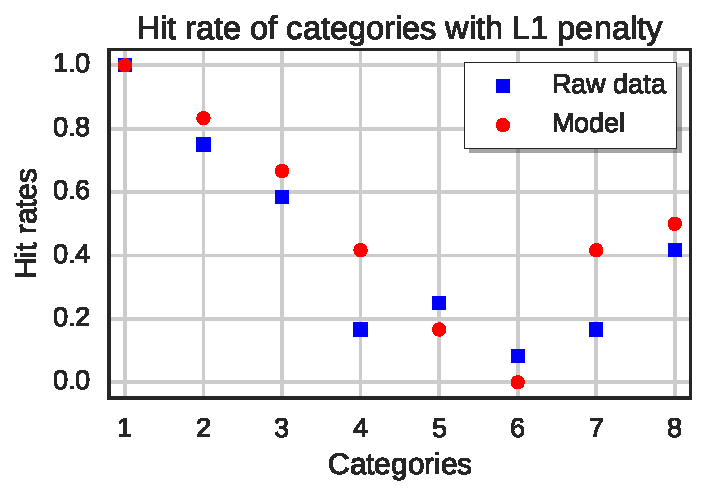
\includegraphics[width=.8\linewidth]{figures/l1_hit_rate_2way}
    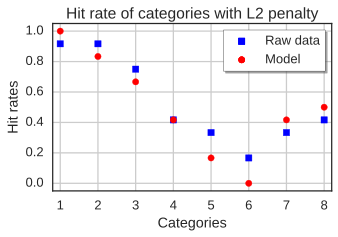
\includegraphics[width=.8\linewidth]{figures/l2_hit_rate_2way}
	\caption{\bf Comparison of actual and inferred states of the macaque dataset.}
	 %using raw data and inferred features for visual category dataset.
	\label{fig:softmax}
\end{figure}

\section*{Experiments}
Code for all algorithms and analyses is available at \url{https://github.com/pearsonlab/spiketopics}.


%
%\section*{Another Section}
%
%Sections can only be used in Articles.  Contributions should be
%organized in the sequence: title, text, methods, references,
%Supplementary Information line (if any), acknowledgements,
%interest declaration, corresponding author line, tables, figure
%legends.
%
%Spelling must be British English (Oxford English Dictionary)
%
%In addition, a cover letter needs to be written with the
%following:
%\begin{enumerate}
% \item A 100 word or less summary indicating on scientific grounds
%why the paper should be considered for a wide-ranging journal like
%\textsl{Nature} instead of a more narrowly focussed journal.
% \item A 100 word or less summary aimed at a non-scientific audience,
%written at the level of a national newspaper.  It may be used for
%\textsl{Nature}'s press release or other general publicity.
% \item The cover letter should state clearly what is included as the
%submission, including number of figures, supporting manuscripts
%and any Supplementary Information (specifying number of items and
%format).
% \item The cover letter should also state the number of
%words of text in the paper; the number of figures and parts of
%figures (for example, 4 figures, comprising 16 separate panels in
%total); a rough estimate of the desired final size of figures in
%terms of number of pages; and a full current postal address,
%telephone and fax numbers, and current e-mail address.
%\end{enumerate}
%
%See \textsl{Nature}'s website
%(\texttt{http://www.nature.com/nature/submit/gta/index.html}) for
%complete submission guidelines.
%
%\begin{methods}
%Put methods in here.  If you are going to subsection it, use
%\verb|\subsection| commands.  Methods section should be less than
%800 words and if it is less than 200 words, it can be incorporated
%into the main text.
%
%\subsection{Method subsection.}
%
%Here is a description of a specific method used.  Note that the
%subsection heading ends with a full stop (period) and that the
%command is \verb|\subsection{}| not \verb|\subsection*{}|.
%
%\end{methods}

%% Put the bibliography here, most people will use BiBTeX in
%% which case the environment below should be replaced with
%% the \bibliography{} command.

% \begin{thebibliography}{1}
% \bibitem{dummy} Articles are restricted to 50 references, Letters
% to 30.
% \bibitem{dummyb} No compound references -- only one source per
% reference.
% \end{thebibliography}

\bibliographystyle{naturemag}
\bibliography{chen_beck_pearson}{}




%\begin{figure}
%%%%\includegraphics{something} % this command will be ignored
%\caption{Each figure legend should begin with a brief title for
%the whole figure and continue with a short description of each
%panel and the symbols used. For contributions with methods
%sections, legends should not contain any details of methods, or
%exceed 100 words (fewer than 500 words in total for the whole
%paper). In contributions without methods sections, legends should
%be fewer than 300 words (800 words or fewer in total for the whole
%paper).}
%\end{figure}


%%
%% TABLES
%%
%% If there are any tables, put them here.
%%

%\begin{table}
%\centering
%\caption{This is a table with scientific results.}
%\medskip
%\begin{tabular}{ccccc}
%\hline
%1 & 2 & 3 & 4 & 5\\
%\hline
%aaa & bbb & ccc & ddd & eee\\
%aaaa & bbbb & cccc & dddd & eeee\\
%aaaaa & bbbbb & ccccc & ddddd & eeeee\\
%aaaaaa & bbbbbb & cccccc & dddddd & eeeeee\\
%1.000 & 2.000 & 3.000 & 4.000 & 5.000\\
%\hline
%\end{tabular}
%\end{table}

\end{document}
